Let $\cX \in \RR^{n_1 \times \cdots \times n_d}$ be a $d$-dimensional array, or tensor, with each mode having length $n_i$. To store a full rank tensor, $n^d$ storage would be required.
A number of tensor factorizations have been developed to reduce this storage cost.
The CANDECOMP/PARAFAC (CP) decomposition \citep{harshman1970foundations,carroll1970analysis} reduces the storage to $O(dnr)$,
reducing the tensor to a sum of $R$ rank-1 weighted outer products:
\begin{align}
\cX^{CP} = \sum_{r=1}^R \lambda_r x_1^r \otimes \cdots \otimes x_d^r
\end{align}
where $x_i^r \in \RR^{n_i}$. Finding the exact CP-rank $r$ is NP-hard, however.
An alternative decomposition decomposes the tensor into sets of matrices and one smaller ``core" tensor.
Generalizing the above,
\begin{align}
\cX^{Tucker} = \cT \otimes_1 G_1 \ldots \otimes_d G_d 
\end{align}
where $\cT \in \RR^{k_1,\ldots,k_d}$ and the outer products are taken along the corresponding dimension.
The size of $\cT$ is defined as the \textit{Tucker rank}, and when $\cX = \cX^{Tucker}$, is analogous to the number of nonzero
eigenvalues for a matrix (tensor of dimension 2).
In this way, it is also considered a \textit{higher-order singular value decomposition},
and algorithms exist for computing it directly.
Unfortunately its space complexity is $O(dnr + r^d)$, reasonable for lower-order tensors
but unsuitable as the order grows.
Hierarchical tensor methods have also proven to be effective in tensor compression \citep{cohen2016expressive, cohen2016convolutional},
and have led to a newer construction with interesting properties.
\begin{figure}
	\centering
	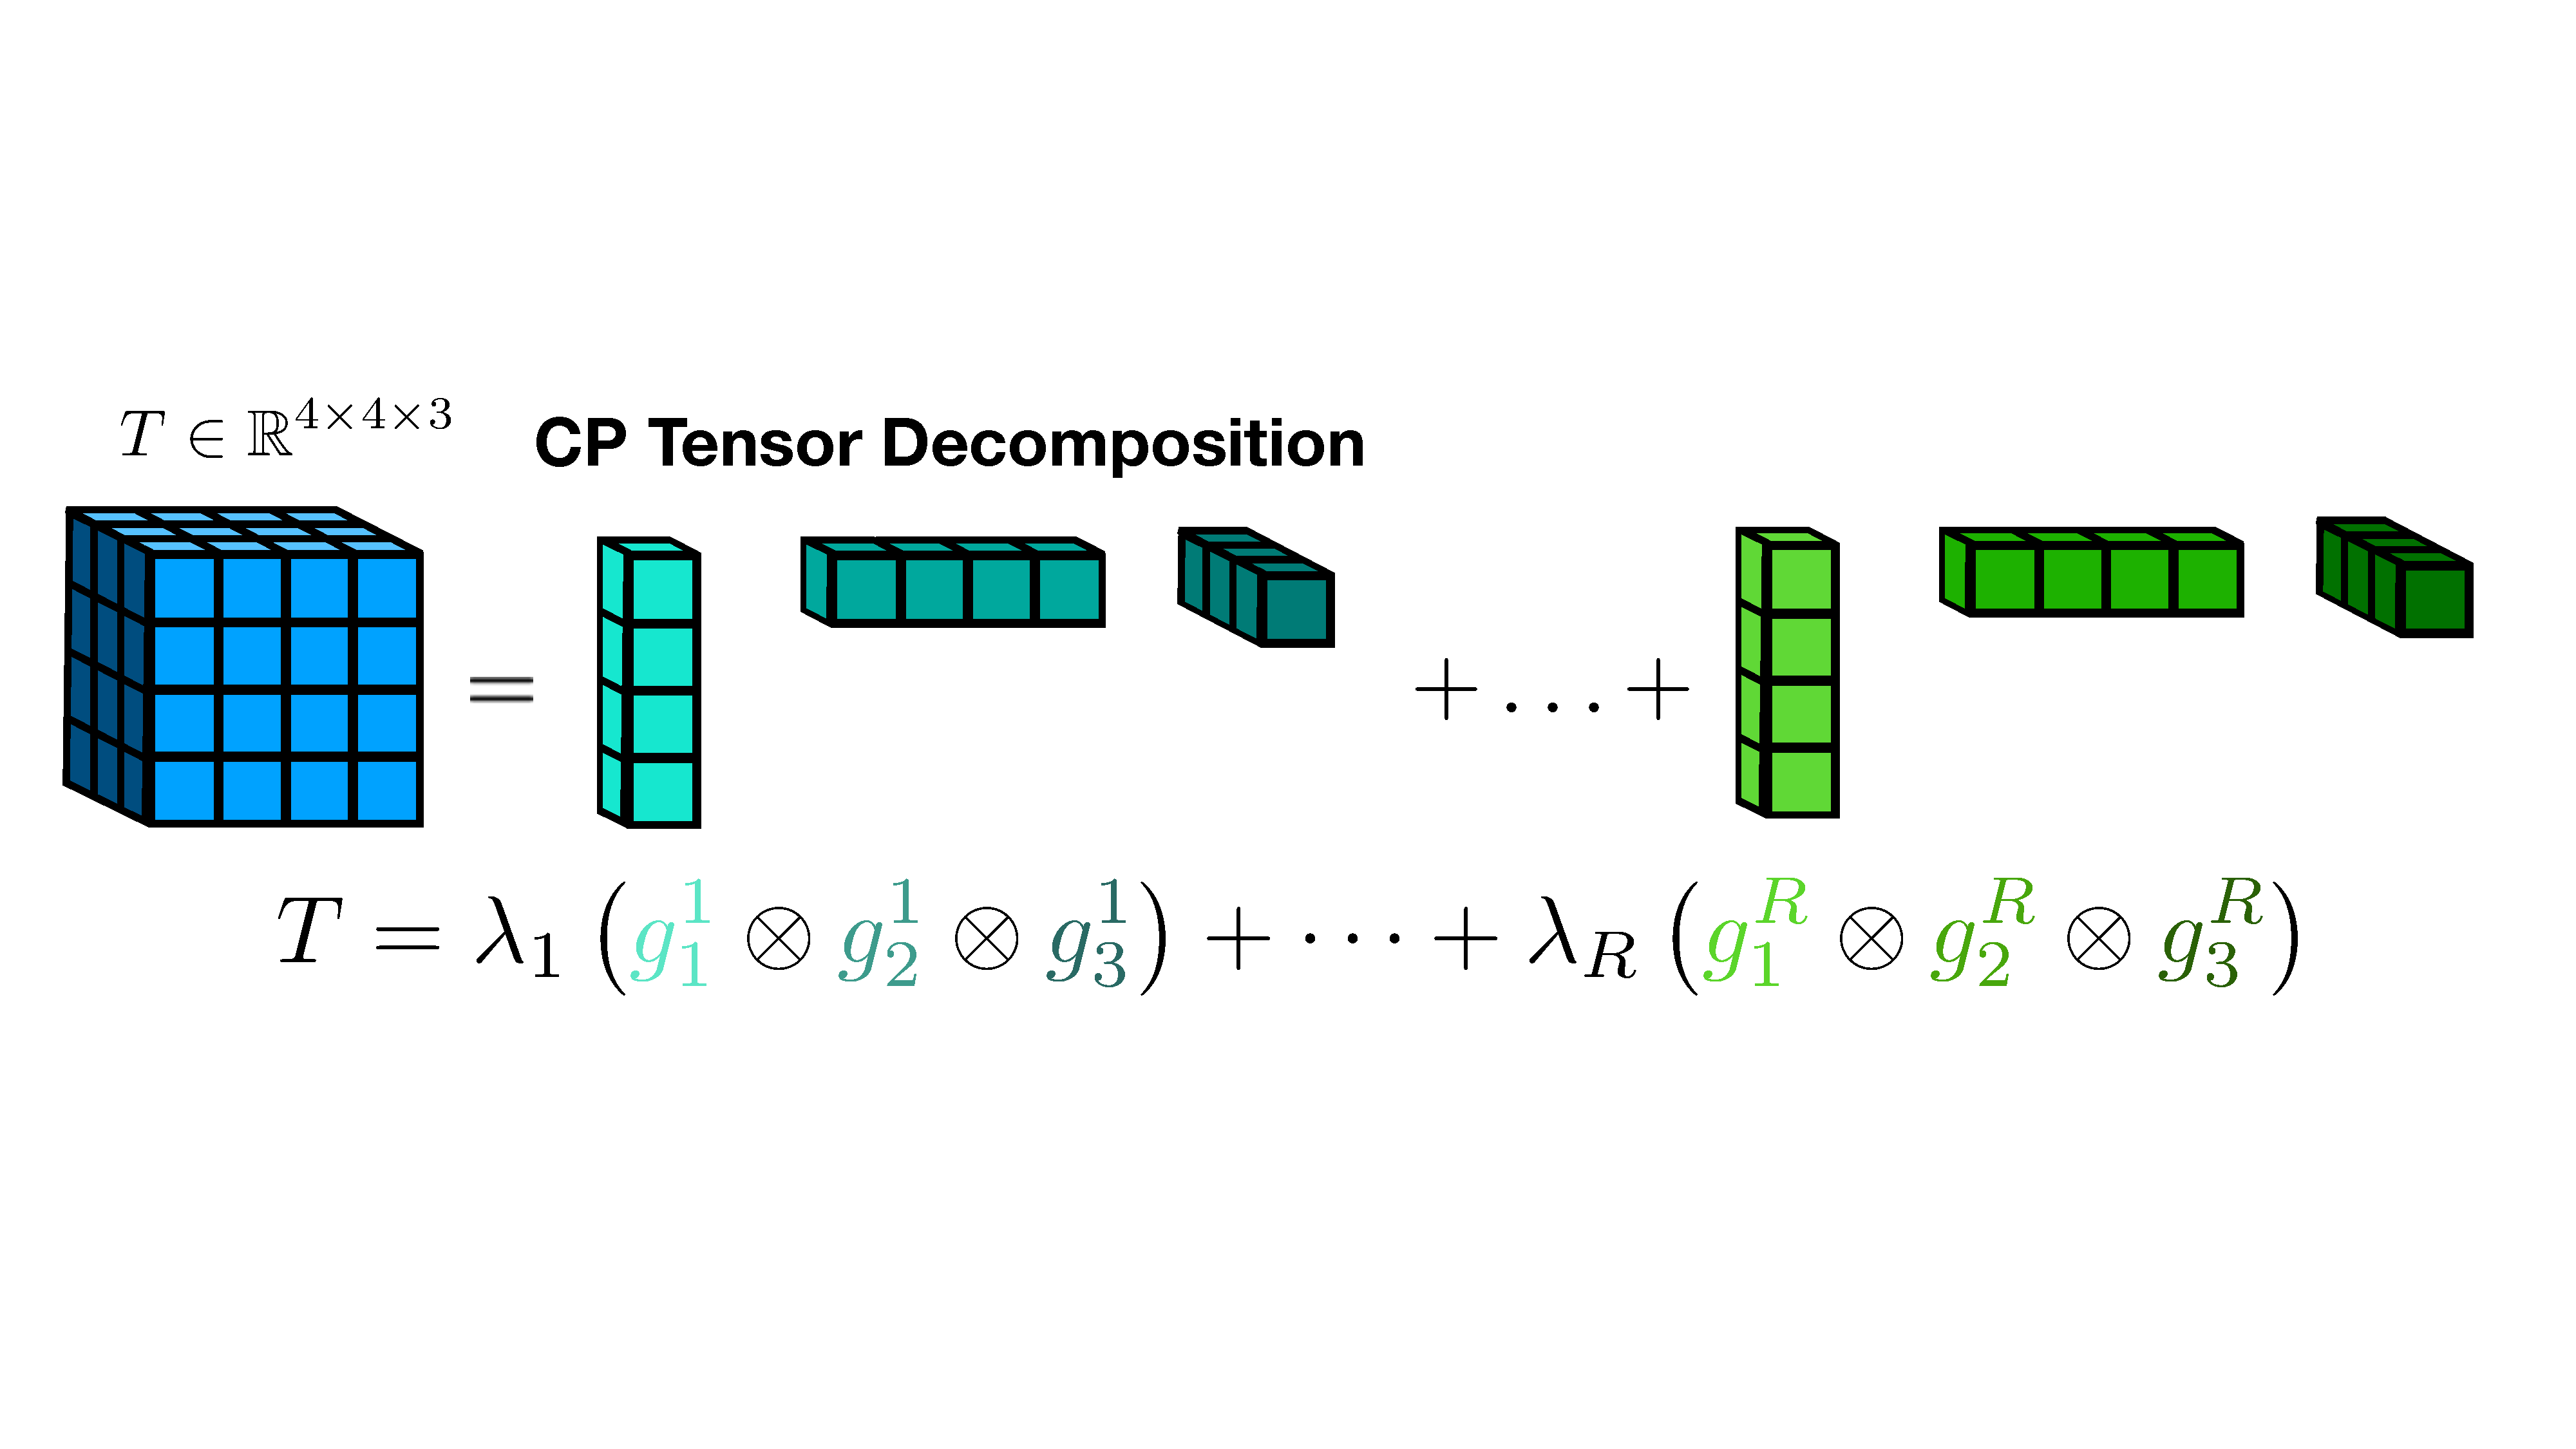
\includegraphics[width=\textwidth,trim={0 9cm 0 10cm},clip]{2_bknd/cpdecomp.pdf}
	\caption[Tensor decompositions]{\label{fig:cp_decomp} CP-style decomposition of an arbitrary tensor.}
\end{figure}

A more recent decomposition, the \textit{Tensor Train} decomposition (TT) \citep{oseledets2011tensor}, defines an element of the tensor as
\begin{align}
\cX(x_1,\ldots,x_d) = A_1(x_1)\cdots A_d(x_d)
\end{align}
where $x_i \in \left\{1,\ldots, n_i\right\}$, and $A_i(x_i) \in \RR^{r_{i-1} \times r_{i}}$ for each $i \in \{1,\ldots,d\}$ are called the \textit{cores} of the tensor train, with $r_0 = r_d = 1$. Equivalently, the full tensor is written as:
\begin{align}\label{eq:fullTT}
	\cX &= \sum_{k_0 = 1}^{r_0} \cdots \sum_{k_d = 1}^{r_d} A_1(k_0,:,k_1) \otimes \cdots \otimes A_d(k_{d-1},:,k_d) 
\end{align}
where $A_i \in \RR^{r_{i-1}\times n_i \times r_i} $. 
This format requires $O(dnr^2)$ storage, but has two major advantages over the CP format. First, finding the TT-rank (the smallest set of $r_i$'s that satisfy the decomposition with equality) of any arbitrary tensor is tractable, and as such all tensors can be efficiently rewritten in the TT format. Second, projecting arbitrary tensors onto the TT format of a fixed rank requires only a set of QR and singular value decompositions \citep{oseledets2011tensor}. This projection, \textit{TT-rounding}, additionally allows for a given TT tensor of some rank to be projected onto the space of TTs with lower rank, and requires $O(dr^3)$ computational complexity. Separately, specific tensor train constructions have recently been identified as forms of general recurrent networks \citep{khrulkov2018generalized}.
\begin{figure}
	\centering
	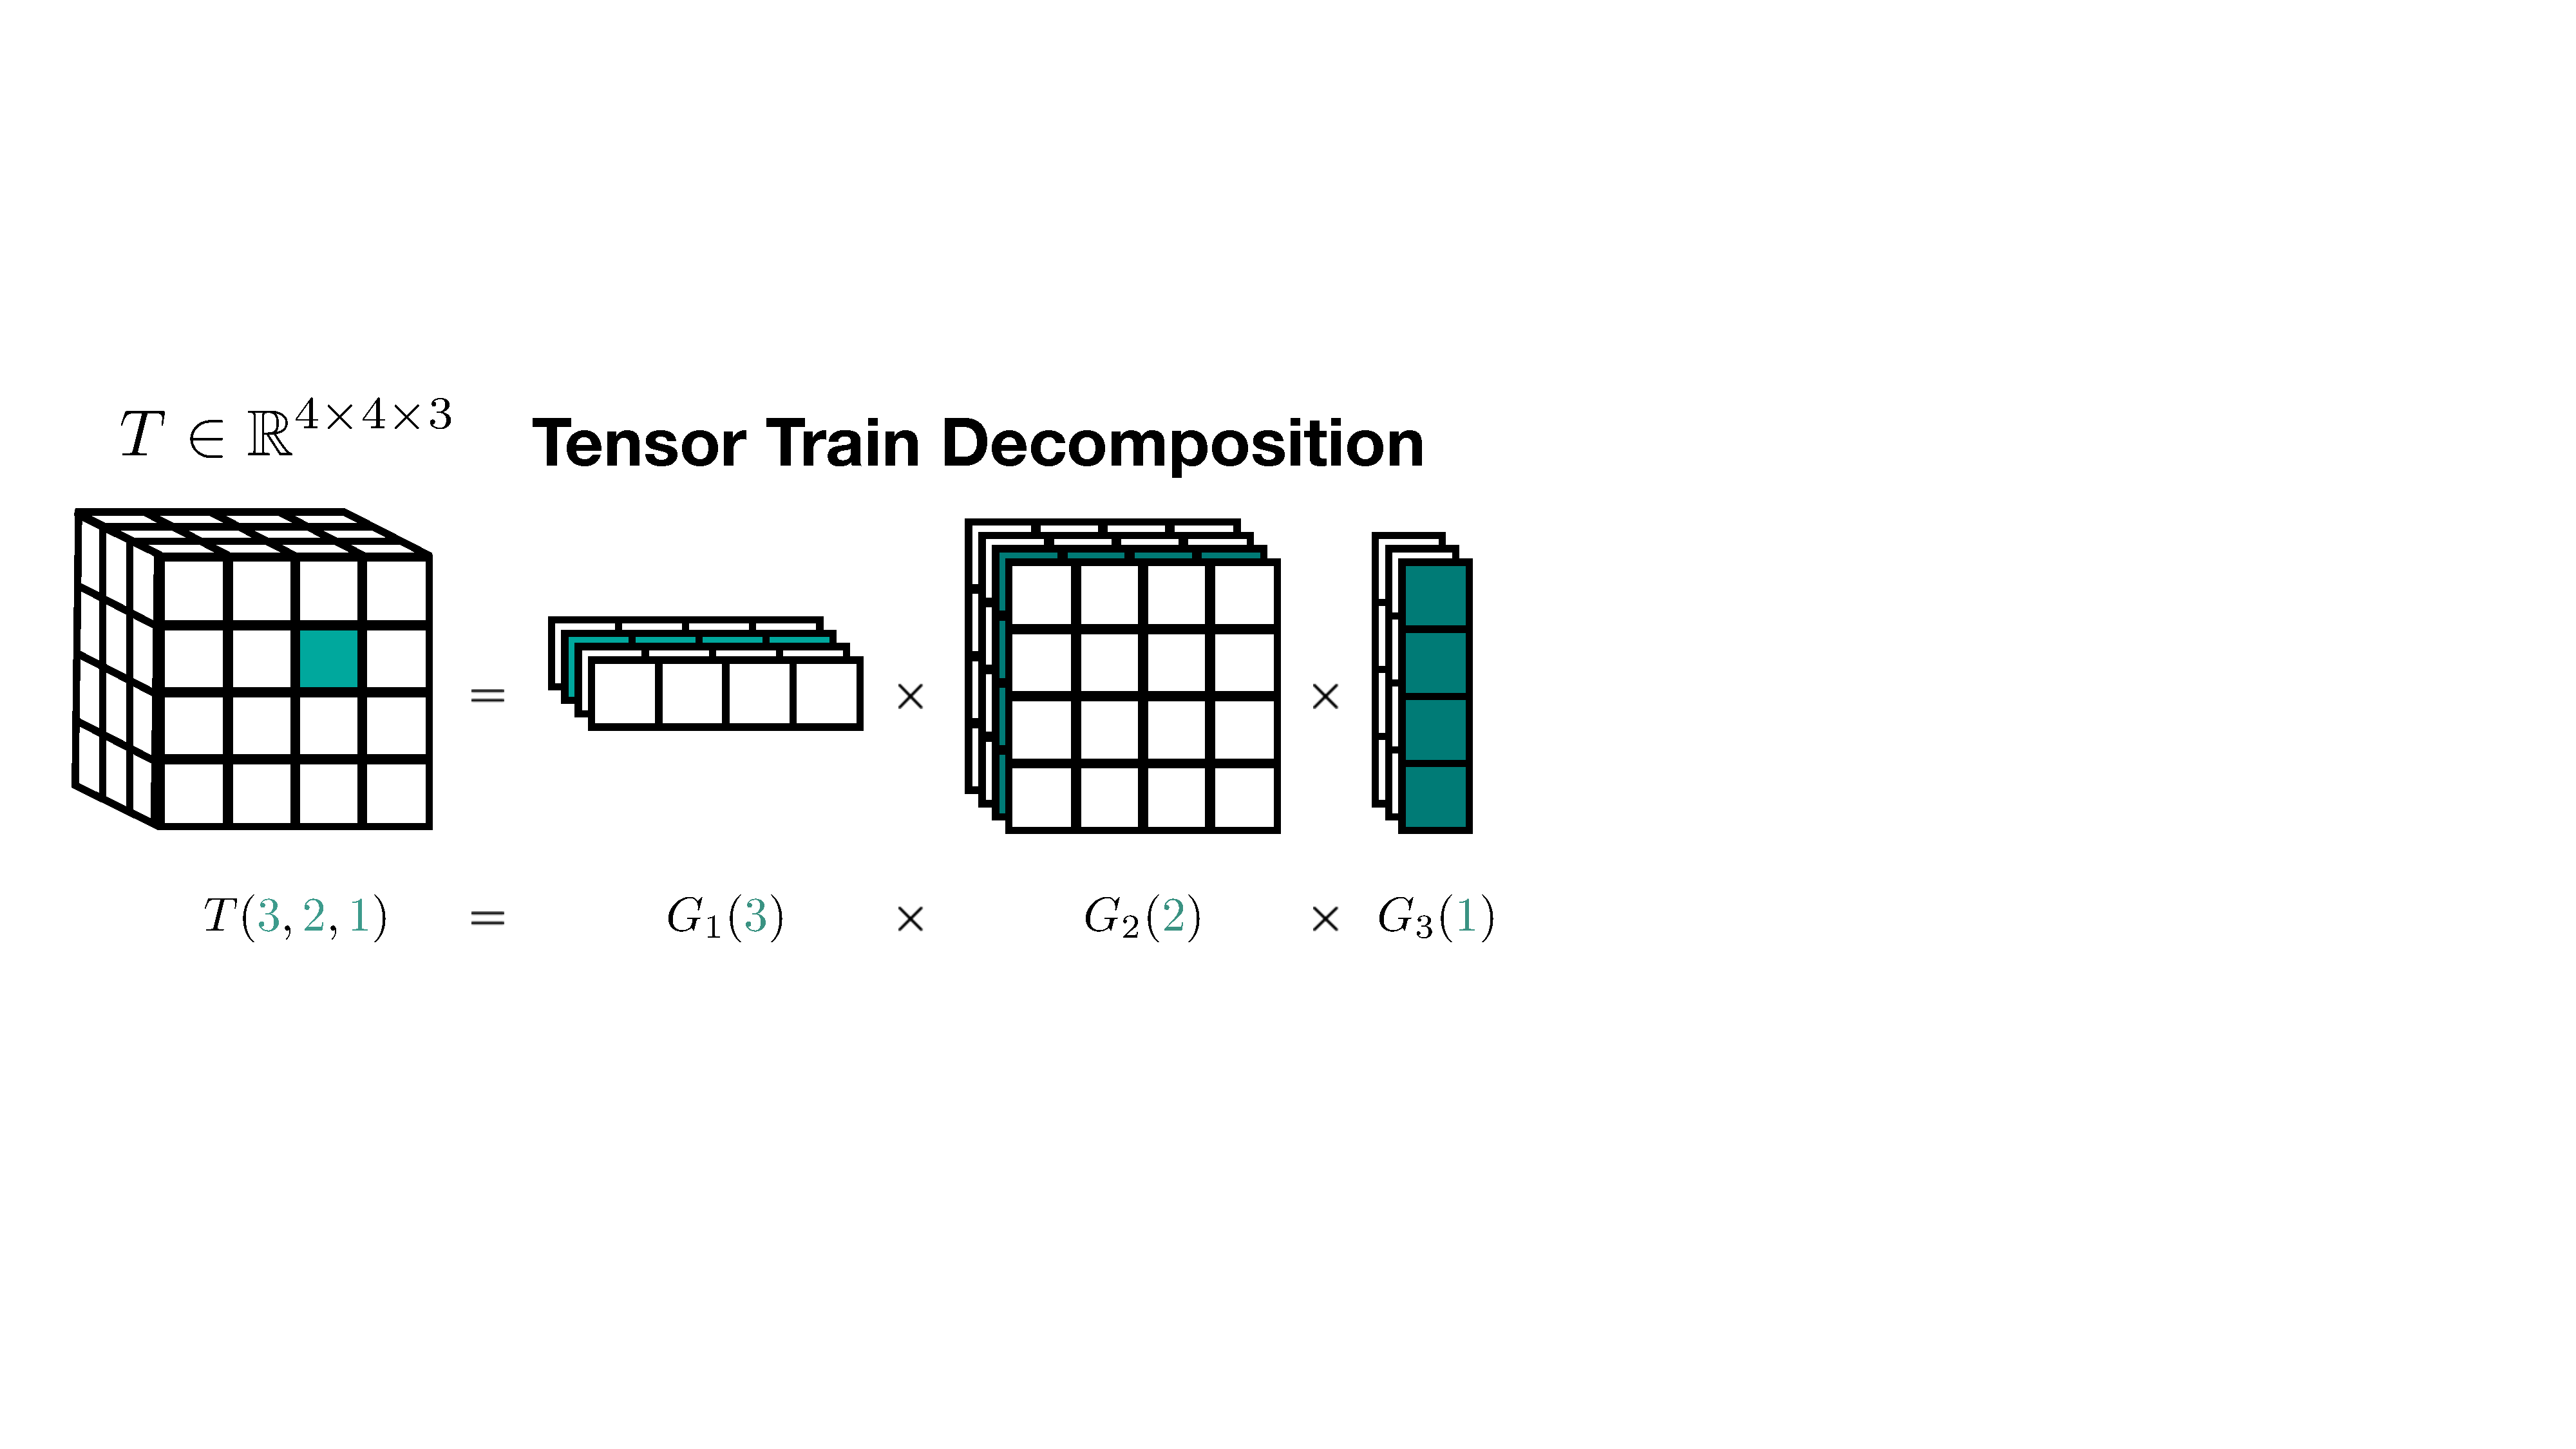
\includegraphics[width=\textwidth,trim={0 12cm 25cm 10cm},clip]{2_bknd/ttdecomp.pdf}
	\caption[Tensor train decomposition]{\label{fig:ttdecomp} Visualization of a tensor train decomposition.}
\end{figure}
We denote a tensor operator $\tG$ as a grouping of tensor modes into an ``input" and ``output" list, such that $\tG \in \RR^{(n_1^{in},\times\ldots\times,n_d^{in}) \times (n_1^{out},\times\ldots\times,n_d^{out})}$. This operator $\tG$ can be seen as the TT representation of a matrix $W \in \RR^{(n_1^i\cdots n_d^i) \times (n_1^o\cdots n_d^o)}$. In \cite{novikov2015tensorizing}, authors use this formulation to directly compress the weight layers in neural networks. Cores in the operator are indexed by both an input and output index, i.e., $A_i(x_i,y_i) \in \RR^{r_{i-1}\times r_i}$, where $x_i \in [1,\ldots,n_i^{in}], y_i \in [1,\ldots,n_i^{out}]$.

Common operations upon tensor trains require \textit{matricizing} the cores of the TT format. Here, we define the left matricization of core $A_i(x_i)$ as $A_i^L \in \RR^{r_{i-1}n_i \times r_i} $ and the right matricization similarly.
Other desirable operations are fully supported by the format as well,
including most linear algebra operations such as summations,
multiplications, Frobenius norms,
and decomposition into the format via an iterative higher-order SVD procedure.
For brevity in this thesis, we refer interested readers
to the original tensor train proposal and citations above.

\subsection{Differential Geometry of Tensor Trains}
Tensor trains with fixed TT-ranks form a Riemannian submanifold of $\RR^{n_1 \times \cdots \times n_d}$ \citep{lubich2015time, holtz2012manifolds}:
\begin{align}\label{eq:riem}
	\cM_r := \{ \cX \in \RR^{n_1 \times \cdots \times n_d} \text{ with TT-ranks\ } r_0,\ldots,r_d\} 
\end{align}
Optimizing a function with respect to a Riemannian manifold-valued variable amounts to computing a free derivative in the ambient space, projecting the gradient to the tangent space of the current iterate, and using the (retraction) exponential map to compute the next iterate.
The authors in \cite{novikov2016exponential} use this procedure to more effectively learn a model of all exponentially many interactions in a linear model.
